\section{Natural language-based vehicle retrieval}
\label{sec:ai_city}
\begin{figure}[!ht]
    \centering
    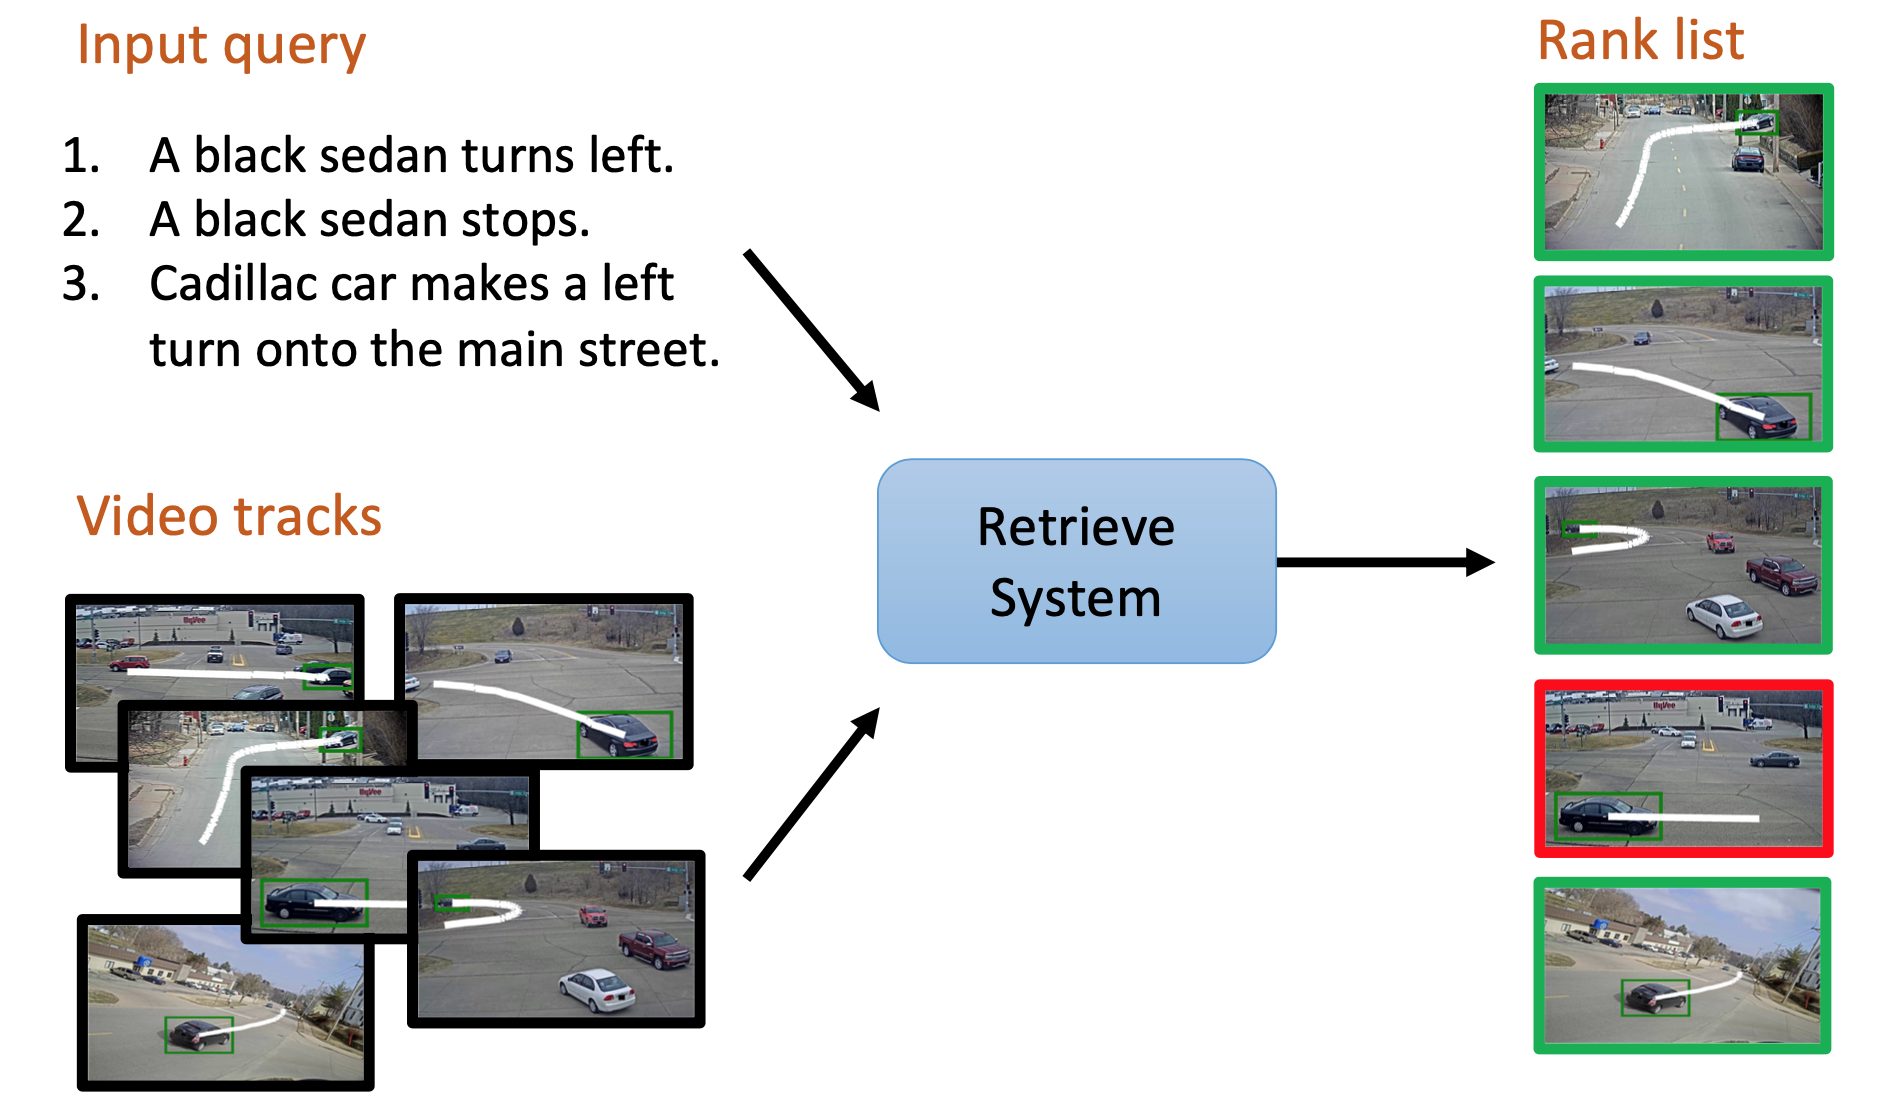
\includegraphics[width=0.9\textwidth]{resources/images/problem_statement.png}
    \caption{NLP-based traffic event retrieval workflow in the AI City Challenge 2021, Track 5.}
    \label{fig:problem_statement}
\end{figure}
In smart cities, Intelligent Traffic Systems (ITS) utilize recorded data and make use of advanced technologies to manage traffic flows, help people and goods move faster. In fact, ITS benefits from insights derived from data captured by sensors. The AI City Challenge \cite{Naphade21AIC21} provides a large video dataset capturing practical traffic scenarios with the intention of integrating intelligent video analytics into real-world deployment. The challenge also provides a scoring system for participants to evaluate their methods in both accuracy and efficiency measures. In 2020, the 5th AI City Challenge is organized with five problem tracks as follows:
\begin{itemize}
    \item \textbf{Multi-class multi-movement vehicle counting using IoT devices}: In this task, participants implement systems to count four-wheel vehicles and freight trucks following a pre-defined movements. The evaluation requires efficient algorithms able to produce accurate results in acceptable runtime. The dataset consists of 31 video clips that capture 20 unique traffic positions.
    \item \textbf{Vehicle re-identification with real and synthetic training data}: The goal of this task is to improve algorithms that identify the same vehicles from different cameras. Dataset provided this year is an extension of the previous version (CityFlowV2-ReID), containing over 85,000 variable-size vehicle images cropped from 46 different cameras. 
    \item \textbf{City-scale multi-target multi-camera vehicle tracking}: Participants perform multi-target multi-camera vehicle tracking on the dataset constructed from 880 distinct annotated vehicle identities, referred to as CityFlowV2. 
    \item \textbf{Traffic anomaly detection}: Teams participating in this track provide algorithms to detect anomalies in camera videos, such as accidents, car crashes or stalled vehicles, etc. The videos in this track are captured at highways and intersections in Iowa, USA. There are 100 videos with a total 18 anomalies for the training set and 150 videos for the test set. 
    \item \textbf{Natural language-based vehicle retrieval}: According to the organizers, this task is the first challenge that utiilizes natural language processing for such a city-scale retrieval problem. In this track, teams were asked to build systems that retrieve appropriate vehicle tracks given natural language descriptions in text. The train dataset contains about 2,500 video-caption pairs while the number is about 150 pairs for the test set (referred to as CityFlow-NL benchmark).
\end{itemize}
In this work, we utilize the Track 5 evaluation platform to experiment and validate our proposed methods on the retrieval task. To keep up with the trending solutions, we discuss some notable solutions for this track at the 5th AI City Challenge. An overview of the mentioned problem is shown in Figure \ref{fig:problem_statement}. \\
\subsection{Impressive solutions for natural language-based vehicle retrieval}
Most existing methods \cite{bai2021connecting, sun2021dun, nguyen2021contrastive, sebastian2021tied, nguyen2021traffic} in Track 5 apply representation learning based modeling for both visual and textual inputs to perform the retrieval task. Experiments indicate that ensembles of different encoder networks provide competitive results for this method.
The 3th solution \cite{park2021keyword} aims to extract descriptive attributes from input query and appearance features from vehicle track to construct a keyword-based retrieval system.

\textbf{Query modeling} \\
The common approach is to utilize pretrained transformer-based models (BERT \cite{devlin2018bert}, RoBERTa \cite{liu2019roberta}) or recurrent units (LSTM \cite{hochreiter1997long}, GRU \cite{cho2014learning}) to embed input query to perform representation semantic matching.
Bai, Shuai, et al \cite{bai2021connecting} enhances model robustness with back-translation augmentation technique.
Park, Eun-Ju, et al \cite{park2021keyword} and Nguyen, Tien-Phat, et al. \cite{nguyen2021traffic} apply conventional natural language tools to analyse the queries, extract useful cues such as vehicle type, color, motion attributes or relationships to neighboring vehicles.

\textbf{Vehicle track modeling} \\ 
Most teams first extract a sequence of frame-level features then apply a sequence model to get final representation of the video track.
Best performing team, Bai, Shuai, et al \cite{bai2021connecting} proposes dual path architecture for video embedding, when one branch aims to extract background information and target vehicle trajectory, the other focuses on the target appearance itself.
Park, Eun-Ju, et al \cite{park2021keyword} intends to build a keyword-based retrieval system that uses target vehicle type, color and movement direction. A color and vehicle classifier trained with cropped images in the given video are used for appearance categorization, while the movement behaviour is modelled from vehicle’s position and velocity vector using trajectory GPS coordinates. 
Through experiments, Park, Eun-Ju, et al \cite{park2021keyword} shows that a combination of searching essential attributes still achieves good results without using any retrieval model.
Nguyen, Tien-Phat, et al. \cite{nguyen2021traffic} applies attribute classification and trajectory-based motion detection to perform re-ranking on final retrieval results and get competitive performance.
\subsection{Conclusion}
Based on the reported results from top teams, we claim that in the vehicle retrieval problem, the targets’ attributes provided by input descriptions are important cues to determine which tracks are mentioned. 
In other words, in the video analytic stage, the algorithm should focus on how the target vehicle looks, by extracting all external attributes, motion patterns and finding out relationships with around vehicles to match with all aspects described in the input queries.
From this point of view, in this work, we propose a retrieval system based on vehicle appearance and motion attributes that achieve best performance on the CityFlow-NL benchmark. In the next sections, we discuss two important tasks utilized to extract vehicle attributes in our proposed method.


